%===============================================================================
% Template for IFAC meeting papers
%===============================================================================
\documentclass{ifacconf}

\usepackage{graphicx}      % include this line if your document contains figures
\usepackage{natbib}        % required for bibliography
\usepackage{amsmath,amssymb}
\usepackage{booktabs}
\usepackage{xcolor}

% Toggle instructional comments (\instrfalse hides all instruction boxes)
\newif\ifinstr \instrfalse

\newcommand{\instr}[1]{%
  \ifinstr
    \par\noindent
    \fcolorbox{orange!80!black}{yellow!20}{%
      \parbox{\dimexpr\linewidth-2\fboxsep-2\fboxrule}{%
        \small\sffamily\color{orange!40!black}%
        \textbf{Instrução:} #1}}%
    \par\medskip
  \fi}

\newcommand{\tamanho}[1]{%
  \ifinstr
    \par\noindent
    \fcolorbox{blue!80!black}{gray!20}{%
      \parbox{\dimexpr\linewidth-2\fboxsep-2\fboxrule}{%
        \small\sffamily\color{black!40!black}%
        \textbf{Tamanho:} #1}}%
    \par\medskip
  \fi}

%===============================================================================
\begin{document}
\begin{frontmatter}

\title{Embedded Neural Approximation of Nonlinear MPC for an Aeropendulum: Experimental Validation\thanksref{footnoteinfo}}

\thanks[footnoteinfo]{The authors thank the Pontifical Catholic University of Paran\'a (PUCPR) and Brazilian funding agencies for supporting this research.}

\author[First]{Felipe Eduardo Marcondes}
\author[First]{Matheus Kale Mendes}
\author[First]{Helon Vicente Hultmann Ayala}

\address[First]{Polytechnic School, Pontifical Catholic University of Paran\'a (PUCPR), Curitiba, PR, Brazil (e-mail: helon.ayala@pucpr.br).}

\begin{abstract}                % Abstract of not more than 250 words.
Nonlinear Model Predictive Control (NMPC) provides superior trajectory tracking and constraint handling for agile mechatronic and Vertical Take-Off and Landing (VTOL) systems, yet its online iterative optimization remains computationally prohibitive for low-cost microcontrollers operating at high sampling rates. This paper presents the end-to-end development, TinyML optimization, and experimental validation of an embedded neural predictive controller for the angular tracking of an instrumented 1-DOF aeropendulum (quarter-drone bench) running at $100\,\mathrm{Hz}$ ($T_s = 10\,\mathrm{ms}$). The nonlinear aerodynamic and gravitational dynamics are identified from closed-loop experimental data using a parsimonious polynomial Nonlinear AutoRegressive with eXogenous inputs (NARX) model selected via the Forward Regression Orthogonal Least Squares (FROLS) algorithm. An Optimal Control Problem (OCP) with a long prediction horizon ($N = 150$) and reference preview is solved offline in CasADi/IPOPT to generate a supervision dataset for a Multilayer Perceptron (MLP) policy. To bridge the Sim-to-Real gap caused by bearing static friction and unmodeled aerodynamic losses, a parallel low-authority residual integral compensator is integrated into the embedded firmware on an ARM Cortex-M4F microcontroller (STM32F446RE). Hardware benchmarks comparing native C compilation against the ST X-CUBE-AI framework show that non-linear weight quantization reduces Flash memory footprint by $86.4\%$ while achieving a deterministic inference latency of $1.82\,\mathrm{ms}$ ($18.2\%$ CPU utilization). Experimental bench trials demonstrate that the hybrid neural controller reduces steady-state bias by over $96\%$ and achieves dynamic tracking RMSE reductions of $69.2\%$ to $81.7\%$ compared to a classical PID controller.
\end{abstract}

\begin{keyword}
Nonlinear model predictive control, neural networks, system identification, NARX models, embedded control, TinyML, aeropendulum.
\end{keyword}

\end{frontmatter}
%===============================================================================

\section{Introduction}

The rapid proliferation of Unmanned Aerial Vehicles (UAVs) and Vertical Take-Off and Landing (VTOL) platforms has intensified the demand for control strategies capable of simultaneously achieving high-precision trajectory tracking, disturbance rejection, and real-time execution on resource-constrained embedded processors \citep{nguyen2020}. In this context, the aeropendulum---or quarter-drone testbench---serves as an effective experimental benchmark that isolates the essential single-degree-of-freedom (1-DOF) rotational dynamics of a VTOL propulsion arm, combining the quadratic aerodynamic thrust of an Electric Ducted Fan (EDF) with nonlinear gravitational restoring torque and bearing friction \citep{job2015,lima2025}.

Nonlinear Model Predictive Control (NMPC) stands out among advanced control methodologies due to its ability to explicitly handle actuator constraints, leverage future reference preview, and anticipate nonlinear plant dynamics \citep{mayne2000,rawlings2017}. However, solving a Nonlinear Programming (NLP) problem online at each sampling instant imposes a severe computational burden. For agile mechatronic systems requiring sampling periods on the order of $T_s = 10\,\mathrm{ms}$ ($100\,\mathrm{Hz}$), iterative numerical solvers frequently exceed the available CPU budget of low-power microcontrollers. While Explicit MPC (EMPC) circumvents online optimization by precomputing piecewise affine (PWA) control laws over polytopic partitions \citep{bemporad2002}, the number of regions grows exponentially with the prediction horizon and state dimension, quickly exhausting the static memory of embedded devices.

To overcome both the latency of online solvers and the combinatorial explosion of EMPC, approximating the implicit MPC policy via Deep Neural Networks (DNNs) has emerged as a compelling paradigm \citep{chen2018approximating,hewing2020learning}. \citet{karg2020} proved that feedforward networks with Rectified Linear Unit (ReLU) activations can exactly represent PWA control laws and approximate nonlinear MPC policies with high fidelity and deterministic memory footprint. Recent theoretical and numerical advances have further addressed statistical and deterministic safety guarantees \citep{hertneck2018,nubert2020safe,alsmeier2024,hose2025approximate}, differentiable predictive control on single-board computers \citep{drgona2022differentiable}, and neural-assisted MPC for quadrotors using onboard GPUs or companion computers \citep{jiang2022,li2022,sanyal2023}.

Despite these advances, a practical technological gap remains regarding end-to-end experimental validations on bare-metal microcontrollers (such as ARM Cortex-M cores) operating at $100\,\mathrm{Hz}$. Whereas studies such as \citet{drgona2022differentiable} deploy policies on Linux-based Raspberry Pi boards at sub-Hertz or slow sampling rates ($T_s = 250\,\mathrm{ms}$), fast mechatronic systems require strict real-time determinism in the millisecond range and must contend with the Sim-to-Real gap induced by static friction and model mismatch when using purely static neural mappings.

The main contributions of this work are threefold:
\begin{enumerate}
    \item An end-to-end data-driven pipeline combining closed-loop polynomial NARX system identification via FROLS with an offline long-horizon NMPC ($N = 150$) featuring future reference preview, distilled into a compact ReLU Multilayer Perceptron (MLP);
    \item A hybrid neural-integral control architecture that pairs the anticipatory feedforward/feedback policy of the MLP with a bounded parallel residual integrator to eliminate steady-state Sim-to-Real bias and mitigate bearing stick-slip friction;
    \item A comprehensive experimental validation on a physical aeropendulum driven by an STM32F446RE microcontroller at $100\,\mathrm{Hz}$, including Software-in-the-Loop (SIL) verification, mirrored comparisons against a tuned PID baseline, and a TinyML trade-off analysis of compiler optimizations and weight compression via ST X-CUBE-AI.
\end{enumerate}

The remainder of this paper is organized as follows. Section~\ref{sec:sysid} describes the experimental bench and the NARX identification procedure. Section~\ref{sec:methodology} formulates the discrete-time NMPC, the MLP imitation learning, and the hybrid residual compensator. Section~\ref{sec:results} presents the experimental results, Sim-to-Real analysis, and embedded TinyML benchmarks. Section~\ref{sec:conclusion} concludes the paper.

%===============================================================================
\section{Experimental Setup and NARX Identification}
\label{sec:sysid}

\subsection{Quarter-Drone Aeropendulum Testbench}

The experimental platform used in this work is the quarter-drone bench developed by \citet{lima2025}. The system consists of a rigid pendulum arm rotating around a horizontal aluminum shaft supported by ball bearings. Propulsion is provided at the tip of the arm by a $50\,\mathrm{mm}$, 11-blade EDF driven by a $4500\,\mathrm{KV}$ brushless outrunner motor and an Electronic Speed Controller (ESC), while adjustable counterweights are mounted on the opposite end of the threaded rod. The angular position $\theta$ is measured with respect to the downward vertical equilibrium ($\theta = 0^\circ$ at rest).

From rotational Newtonian mechanics, the conceptual continuous-time dynamics are governed by
\begin{equation} \label{eq:physical_ode}
J\ddot{\theta} + b\dot{\theta} + (m_1 L_1 - m_2 L_2)g\sin(\theta) = \tau(u),
\end{equation}
where $J$ is the total moment of inertia, $b$ is the viscous damping coefficient, $m_1, L_1$ and $m_2, L_2$ are the masses and lever arms of the thruster and counterweight, respectively, $g$ is gravitational acceleration, and $\tau(u)$ is the aerodynamic torque generated by the normalized PWM command $u \in [0, 100]\%$. Because first-principles parameterization of (\ref{eq:physical_ode}) struggles to capture EDF aerodynamic hysteresis, duct recirculation, and bearing friction across wide angular excursions, we adopt a data-driven discrete-time nonlinear identification approach.

The embedded processing unit is an STM32 Nucleo-F446RE board featuring a 32-bit ARM Cortex-M4F microcontroller clocked at $180\,\mathrm{MHz}$, equipped with a single-precision hardware Floating-Point Unit (FPU), $512\,\mathrm{KB}$ of Flash memory, and $128\,\mathrm{KB}$ of SRAM. Angular sensing is performed at $f_s = 100\,\mathrm{Hz}$ ($T_s = 10\,\mathrm{ms}$) using an InvenSense ICM-20948 9-axis MEMS Inertial Measurement Unit (IMU) communicating via $\mathrm{I}^2\mathrm{C}$ in Fast Mode ($400\,\mathrm{kHz}$) with Direct Memory Access (DMA) and a digital low-pass filter (DLPF) cutoff of $51.2\,\mathrm{Hz}$. A complementary filter fuses accelerometer and gyroscope readings to estimate $\theta(k)$ in real time, while telemetry is streamed to a host PC via UART DMA at $500\,\mathrm{kbaud}$.

\subsection{Closed-Loop Excitation and Data Partitioning}

Due to the lightly damped nature of the pendulum ($\zeta \approx 0.175$, natural frequency $f_n \approx 0.40\,\mathrm{Hz}$) and the absence of mechanical end-stops, open-loop excitation is unsafe. Consequently, identification experiments were conducted in closed loop using a preliminary digital PID controller with gains $K_p = 0.5793$, $K_i = 0.6647$, and $K_d = 0.2000$, synthesized via frequency-response tuning around $\theta_0 = 40^\circ$ with trapezoidal integration, derivative-on-measurement, and back-calculation anti-windup \citep{astrom1995}.

To excite the nonlinear dynamics across the full operating envelope $\theta \in [0^\circ, 120^\circ]$ up to the mechanical bandwidth $f_{\max} = 0.50\,\mathrm{Hz}$, 24 closed-loop experiments were designed around two equilibrium operating points ($\theta_0 = 45^\circ$ and $\theta_0 = 60^\circ$), comprising four signal classes \citep{ljung1999}: (i)~random-phase multisines ($f_{\max} \in \{0.30, 0.40, 0.50\}\,\mathrm{Hz}$, crest factor $\mathrm{CF} \le 1.8$); (ii)~swept-sine chirps ($0.05$ to $0.50\,\mathrm{Hz}$, amplitudes $\pm 25^\circ$ to $\pm 60^\circ$); (iii)~Amplitude Pseudo-Random Binary Sequences (APRBS, random dwell times in $[2.0, 4.0]\,\mathrm{s}$); and (iv)~multi-level fixed steps.

To prevent overfitting, model estimation used exclusively the 6 most demanding trials (highest bandwidth $f_{\max} = 0.50\,\mathrm{Hz}$ and largest excursions in multisine, chirp, and APRBS at both $45^\circ$ and $60^\circ$). All remaining 18 trials with intermediate frequencies and distinct step profiles were strictly held out for independent Free-Run (FR) cross-validation.

\subsection{Polynomial NARX Structure Selection via FROLS}

The discrete-time SISO polynomial NARX model represents the one-step-ahead output prediction $\hat{y}(k)$ as a linear-in-the-parameters expansion \citep{billings2013,aguirre2015}:
\begin{equation} \label{eq:narx_model}
\hat{y}(k) = \sum_{m=1}^{M} \hat{\theta}_m p_m\bigl(y(k-1),\dots,y(k-n_y),u(k-1),\dots,u(k-n_u)\bigr),
\end{equation}
where $p_m(\cdot)$ are monomials of degree up to $\ell$ formed by lagged outputs $y(k-i)$ and inputs $u(k-j)$, and $\hat{\theta}_m$ are constant parameters. Setting maximum lags $n_y = 15$ ($150\,\mathrm{ms}$), $n_u = 15$ ($150\,\mathrm{ms}$), and polynomial degree $\ell = 2$ yields $M_{\mathrm{total}} = (n_y + n_u + \ell)! / [(n_y + n_u)!\,\ell!] = 496$ candidate regressors.

To avoid ill-conditioning and unstable free-run recursion, the Forward Regression Orthogonal Least Squares (FROLS) algorithm \citep{chen1989} was applied using the Error Reduction Ratio ($\mathrm{ERR}$) criterion:
\begin{equation} \label{eq:err}
[\mathrm{ERR}]_i = \frac{g_i^2 w_i^\top w_i}{y^\top y} \times 100\%, \qquad g_i = \frac{w_i^\top y}{w_i^\top w_i},
\end{equation}
where $w_i$ are orthogonalized basis vectors. Greedy selection was truncated at $M = 10$ terms, yielding the parsimonious model reported in Table~\ref{tb:narx_terms}.

\begin{table}[tb]
\begin{center}
\caption{Selected polynomial NARX regressors and estimated coefficients ($M = 10$).}\label{tb:narx_terms}
\begin{tabular}{lr@{\hspace{1.2cm}}lr}
\toprule
\textbf{Regressor} & \textbf{Coefficient ($\hat{\theta}_m$)} & \textbf{Regressor} & \textbf{Coefficient ($\hat{\theta}_m$)} \\
\midrule
$y(k-1)$       & $+1.4230$             & $y(k-1)^2$     & $+6.9 \times 10^{-6}$  \\
$y(k-2)$       & $-0.2120$             & $u(k-3)u(k-6)$ & $-9.3 \times 10^{-7}$  \\
$y(k-4)$       & $-0.1568$             & $u(k-6)u(k-9)$ & $+1.77 \times 10^{-5}$ \\
$y(k-10)$      & $-0.0944$             & $u(k-3)u(k-15)$& $+9.3 \times 10^{-6}$  \\
$y(k-15)$      & $+0.0388$             & $\mathrm{Constant}$ & $-0.0059$         \\
\bottomrule
\end{tabular}
\end{center}
\end{table}

Notably, FROLS automatically selected exclusively quadratic delayed input products $u(k-i)u(k-j)$, which is physically consistent with the aerodynamic thrust law of ducted fans ($\tau \propto \omega^2$). Because this quadratic input structure induces even symmetry $F(y, -u) = F(y, u)$, a lower bound $u \ge 0$ is enforced during NMPC synthesis.

Model qualification was conducted strictly in Free-Run ($\mathrm{FR}$) simulation, where $\hat{y}_{\mathrm{FR}}(k)$ is propagated open-loop over thousands of steps using only its own past predictions $\hat{y}_{\mathrm{FR}}(k-i)$ and the experimental input sequence $u(k-j)$. Across the held-out validation sets, the 10-term NARX model achieved $\mathrm{RMSE} = 4.685^\circ$ on the $130\,\mathrm{s}$ validation multisine, $\mathrm{RMSE} = 5.678^\circ$ ($\mathrm{MAE} = 4.238^\circ$, $\mathrm{FIT} = 74.7\%$, $R^2 = 0.936$) on the $125\,\mathrm{s}$ multi-step sequence (Fig.~\ref{fig:narx_steps}), and $\mathrm{RMSE} = 6.270^\circ$ ($\mathrm{FIT} = 72.2\%$, $R^2 = 0.922$) on the $\pm 35^\circ$ chirp test, exhibiting zero phase drift and high structural stability.

\begin{figure}[tb]
\begin{center}
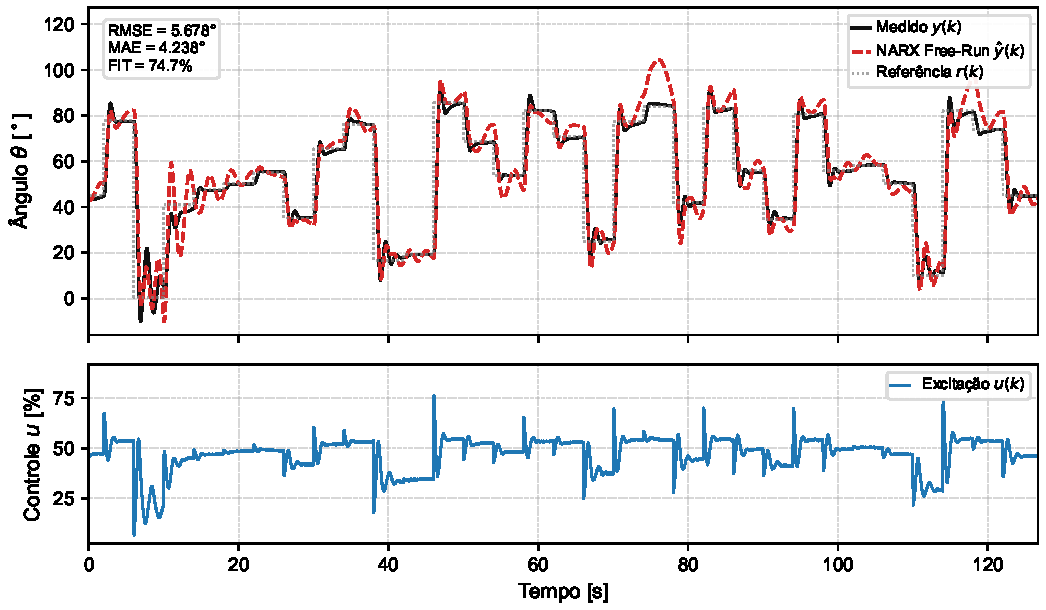
\includegraphics[width=8.4cm]{img/narx_val_steps.pdf}
\caption{Free-run validation of the 10-term NARX model over an independent $125\,\mathrm{s}$ multi-step trial around $45^\circ$ ($\mathrm{RMSE} = 5.678^\circ$, $\mathrm{FIT} = 74.7\%$).}
\label{fig:narx_steps}
\end{center}
\end{figure}

%===============================================================================
\section{Embedded Neural Approximate NMPC}
\label{sec:methodology}

\subsection{Discrete-Time NMPC Formulation with Preview}

To embed the NARX predictor (\ref{eq:narx_model}) into a canonical discrete-time state-space framework at $T_s = 10\,\mathrm{ms}$, we define the augmented shift-register state vector $x_k \in \mathbb{R}^{30}$:
\begin{equation} \label{eq:narx_state}
x_k = \bigl[y(k-1),\dots,y(k-15),\, u(k-1),\dots,u(k-15)\bigr]^\top.
\end{equation}
The state transition $x_{k+j+1|k} = F(x_{k+j|k}, u_{k+j})$ shifts the historical buffers and inserts the one-step NARX prediction $y_{k+j|k} = \mathcal{M}_{\mathrm{NARX}}(x_{k+j|k})$ and applied input $u_{k+j}$ without numerical integration truncation errors.

At each sampling instant $k$, given the current state $x_k$ and a future reference trajectory preview $\mathbf{r}_k = [r_k, r_{k+1}, \dots, r_{k+N-1}]^\top$ over horizon $N = 150$ ($1.50\,\mathrm{s}$, approximately four times the natural oscillation period of the pendulum), the Optimal Control Problem (OCP) minimizes
\begin{subequations} \label{eq:ocp}
\begin{align}
\min_{U_k} \quad & J(x_k, U_k, \mathbf{r}_k) = \sum_{j=0}^{N-1} \Bigl[ q_y\bigl(y_{k+j|k} - r_{k+j}\bigr)^2 \nonumber\\[-3pt]
                 & \hspace{2.7cm} + r_u u_{k+j}^2 + r_{\Delta u} (\Delta u_{k+j})^2 \Bigr] \label{eq:ocp_cost}\\
\textrm{s.t.} \quad & x_{k|k} = x_k, \quad x_{k+j+1|k} = F(x_{k+j|k}, u_{k+j}), \\
                    & u_{\min} \le u_{k+j} \le u_{\max}, \quad \forall j \in \{0,\dots,N-1\},
\end{align}
\end{subequations}
where $U_k = \{u_k, \dots, u_{k+N-1}\}$, $\Delta u_{k+j} = u_{k+j} - u_{k+j-1}$ penalizes actuator slew rate (with $u_{k-1}$ read directly from $x_k$), and the input bounds are $u_{\min} = 0\%$ and $u_{\max} = 100\%$ (capped at $80\%$ in bench firmware for thermal protection). The weighting parameters were tuned to $q_y = 1000.0$, $r_u = 0.1$, and $r_{\Delta u} = 50000.0$, where the strong $\Delta u$ penalty acts as a dynamic smoothing filter against high-frequency ESC switching. Under the sufficiently long horizon $N = 150$, explicit terminal set constraints are omitted to prevent artificial solver infeasibility during abrupt reference steps \citep{rawlings2017}. By the receding-horizon principle, the implicit NMPC policy applies $\kappa_N(x_k, \mathbf{r}_k) := u_k^*$.

The OCP (\ref{eq:ocp}) was formulated symbolically in CasADi \citep{andersson2019} using algorithmic differentiation and solved via IPOPT. As shown in Fig.~\ref{fig:mpc_time}, evaluating the exact NMPC on a desktop CPU requires $90$ to $120\,\mathrm{ms}$ per step on average, with a cold-start peak of $458\,\mathrm{ms}$ and transient peaks of $220$ to $333\,\mathrm{ms}$ during step transitions---exceeding the $T_s = 10\,\mathrm{ms}$ real-time deadline by a factor of $10\times$ to $45\times$.

\begin{figure}[tb]
\begin{center}
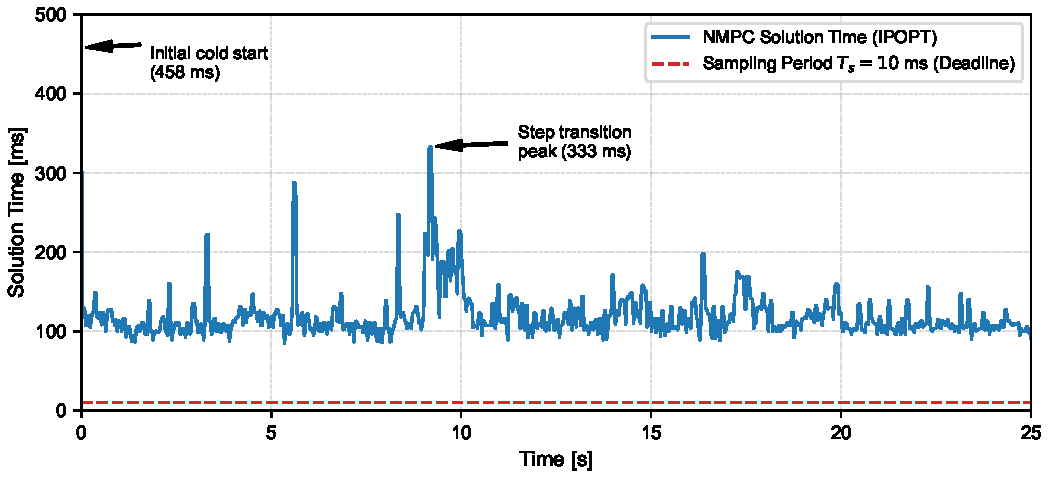
\includegraphics[width=8.4cm]{img/mpc_tempo.pdf}
\caption{Per-step solution time of the nominal NMPC (CasADi/IPOPT) compared against the $T_s = 10\,\mathrm{ms}$ real-time sampling deadline.}
\label{fig:mpc_time}
\end{center}
\end{figure}

\subsection{Imitation Learning via Preview-Augmented MLP}

To distill the optimal policy $\kappa_N$ into a constant-time embedded mapping, the nominal NMPC was simulated in closed loop over a rich $187\,\mathrm{s}$ reference profile ($M_{\mathrm{data}} = 18,700$ samples at $100\,\mathrm{Hz}$) combining multisines (up to $0.50\,\mathrm{Hz}$), chirps, and steps spanning $[12^\circ, 110^\circ]$. At each step $k$, we record the supervision pair $(z_k, u_k^*)$, where the feature vector $z_k \in \mathbb{R}^{130}$ concatenates the $n_y = 15$ past outputs, $n_u = 15$ past inputs, and $N_{\mathrm{prev}} = 100$ future reference steps ($1.0\,\mathrm{s}$ of anticipatory preview):
\begin{equation} \label{eq:mlp_input}
z_k = \bigl[x_k^\top,\; r_k,\, r_{k+1},\, \dots,\, r_{k+99}\bigr]^\top \in \mathbb{R}^{130}.
\end{equation}

After $Z$-score standardization of $z_k$, a feedforward MLP with topology $130 \to 128 \to 128 \to 1$ ($33,665$ trainable parameters, ReLU hidden activations, and linear output) was trained in PyTorch \citep{paszke2019} minimizing the Mean Squared Error $\mathcal{L}_{\mathrm{MSE}} = \frac{1}{B}\sum_{i=1}^B (\hat{u}_i - u_i^*)^2$ via Adam ($\alpha = 10^{-3}$, weight decay $10^{-5}$, batch size $64$, \texttt{ReduceLROnPlateau}, and early stopping). The network converged in fewer than 5 epochs, achieving $R^2 = 0.999$ across training, validation, and test splits.

\subsection{Hybrid Neural-Integral Control Architecture}

While the MLP accurately replicates the dynamic and anticipatory behavior of the NMPC, a purely static neural network lacks an internal state (pole at the origin). When deployed on the physical aeropendulum, unmodeled effects---specifically ball-bearing static friction (\emph{stick-slip}), aerodynamic recirculation losses at high angles, and slight thermal drift in motor thrust---manifest as persistent steady-state offsets.

To overcome this limitation while preserving the fast nonlinear preview policy of the network, we propose a parallel hybrid neural-integral architecture:
\begin{equation} \label{eq:hybrid_law}
u[k] = u_{\mathrm{ANN}}[k] + u_{i,\mathrm{res}}[k],
\end{equation}
where $u_{\mathrm{ANN}}[k] = \mathrm{MLP}(z_k)$ is the neural inference and $u_{i,\mathrm{res}}[k]$ is a low-authority residual integrator discretized via Tustin's trapezoidal rule with symmetrical anti-windup clamping:
\begin{subequations} \label{eq:residual_integrator}
\begin{align}
\tilde{u}_{i,\mathrm{res}}[k] &= u_{i,\mathrm{res}}[k-1] + K_{i,\mathrm{res}}\frac{T_s}{2}\bigl(e[k] + e[k-1]\bigr), \\
u_{i,\mathrm{res}}[k] &= \mathrm{sat}\bigl(\tilde{u}_{i,\mathrm{res}}[k],\, -U_{i,\max},\, +U_{i,\max}\bigr),
\end{align}
\end{subequations}
with tracking error $e[k] = r[k] - y[k]$, residual integral gain $K_{i,\mathrm{res}} = 0.20$, and authority bound $U_{i,\max} = 10.0\%$. Restricting $U_{i,\max} = 10.0\%$ guarantees that the MLP retains at least $90\%$ of the control authority during agile transients while the residual integrator smoothly supplies the exact bias needed to break static friction and eliminate steady-state offset.

%===============================================================================
\section{Experimental Results and Analysis}
\label{sec:results}

\subsection{Triad Validation and Sim-to-Real Gap Mitigation}

To systematically separate numerical implementation effects from physical plant mismatch, the closed-loop control law was evaluated across a three-stage triad: (i)~ideal Python simulation (\texttt{float64}); (ii)~Software-in-the-Loop (SIL) on the STM32F446RE executing the compiled C neural policy and the NARX plant in \texttt{float32} at $100\,\mathrm{Hz}$; and (iii)~real-time physical bench operation. A standardized $75\,\mathrm{s}$ protocol was adopted: $0\text{--}5\,\mathrm{s}$ soft-start under baseline PID, $5\text{--}70\,\mathrm{s}$ active neural control window (used for all RMSE and bias metrics), and $70\text{--}75\,\mathrm{s}$ return to baseline PID. Three independent validation profiles were tested:
\begin{itemize}
    \item \textbf{Scenario 1 (Multisine + Steps):} Superimposed multisine, high-frequency chirp ($40\text{--}50\,\mathrm{s}$), and rectangular steps;
    \item \textbf{Scenario 2 (Random Steps):} Abrupt multi-level steps up to $95^\circ$;
    \item \textbf{Scenario 3 (Smooth Sine):} Wide-amplitude sinusoidal wave with gradual velocity zero-crossings.
\end{itemize}

Table~\ref{tb:triad_rmse} summarizes the tracking performance across all environments for both the Nominal (pure MLP) and Hybrid (MLP + residual integrator) configurations.

\begin{table*}[tb]
\begin{center}
\caption{Closed-loop tracking RMSE and steady-state bias across the validation triad ($5.0\,\mathrm{s}$ to $70.0\,\mathrm{s}$ active window).}\label{tb:triad_rmse}
\begin{tabular}{lccccccc}
\toprule
\textbf{Validation Scenario} & \textbf{Python ($^\circ$)} & \textbf{SIL Nom. ($^\circ$)} & \textbf{SIL Hyb. ($^\circ$)} & \textbf{Bench Nom. ($^\circ$)} & \textbf{Bench Hyb. ($^\circ$)} & \textbf{Bench RMSE Red.} & \textbf{Bench Bias Reduction} \\
\midrule
1. Multisine + Steps & $1.49$ & $2.48$ & $1.53$ & $3.13$ & $\mathbf{2.20}$ & $\mathbf{-29.8\%}$ & $+2.29^\circ \to \mathbf{+0.03^\circ}$ ($-98.8\%$) \\
2. Random Steps      & $3.63$ & $3.78$ & $3.38$ & $4.61$ & $\mathbf{3.60}$ & $\mathbf{-21.8\%}$ & $+2.67^\circ \to \mathbf{+0.07^\circ}$ ($-97.5\%$) \\
3. Smooth Sine       & $1.34$ & $1.49$ & $0.62$ & $3.55$ & $\mathbf{1.75}$ & $\mathbf{-50.8\%}$ & $+2.13^\circ \to \mathbf{+0.08^\circ}$ ($-96.2\%$) \\
\bottomrule
\end{tabular}
\end{center}
\end{table*}

Comparing Python simulation against STM32 SIL confirms high numerical fidelity: Pearson correlation between \texttt{float64} Python trajectories and \texttt{float32} Cortex-M4F SIL trajectories exceeded $r > 0.998$ in all scenarios. Notably, the preview capability learned by the MLP is clearly observed in Scenario~2, where the control signal and pendulum arm initiate movement fractions of a second prior to step transitions, proactively compensating for rotational inertia.

When deploying the Nominal MLP on the physical bench, a consistent steady-state bias between $+2.13^\circ$ and $+2.67^\circ$ emerged due to Sim-to-Real model mismatch, alongside flat dead-zones at velocity zero-crossings in Scenario~3 caused by unmodeled ball-bearing static friction. As illustrated in Figs.~\ref{fig:bench_hyb_val1} and \ref{fig:bench_hyb_val3}, activating the hybrid residual integrator (\ref{eq:hybrid_law}) virtually eliminated steady-state bias---reducing mean offset by $98.8\%$ in Scenario~1 ($+0.03^\circ$) and $97.5\%$ in Scenario~2 ($+0.07^\circ$)---while smoothly accumulating torque at velocity reversals to overcome stick-slip friction, cutting the sinusoidal RMSE in Scenario~3 by more than half ($3.55^\circ \to 1.75^\circ$, a $50.8\%$ reduction) without inducing actuator chatter.

\begin{figure}[tb]
\begin{center}
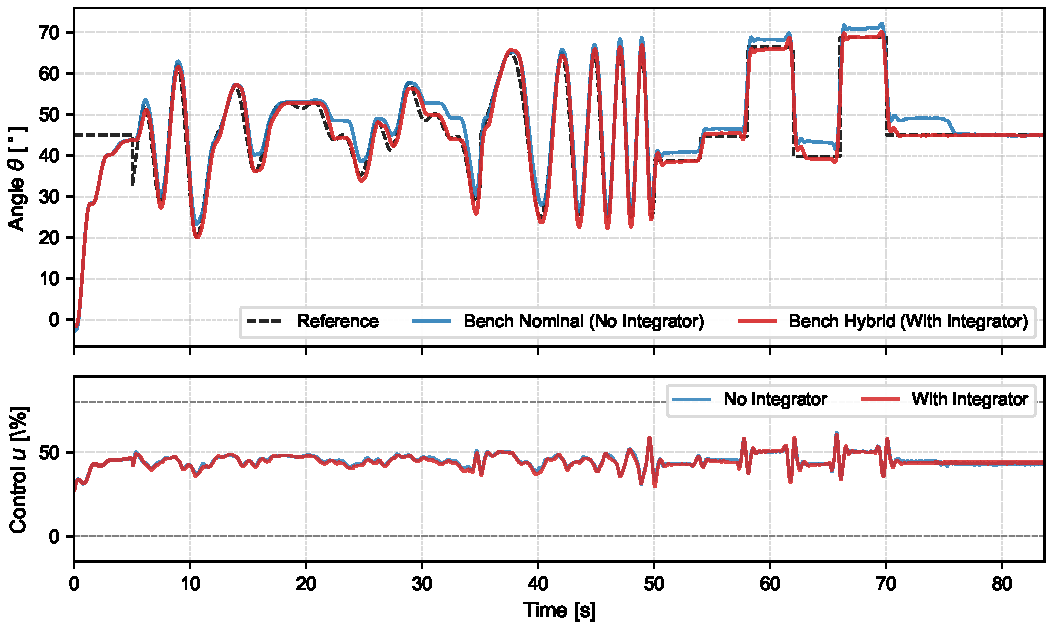
\includegraphics[width=8.4cm]{img/comparacao_hibrido_val1.pdf}
\caption{Physical bench response for Scenario 1 (Multisine + Steps): Nominal MLP vs. Hybrid Neural-Integral controller ($\mathrm{RMSE}$ reduced from $3.13^\circ$ to $2.20^\circ$, bias reduced by $98.8\%$).}
\label{fig:bench_hyb_val1}
\end{center}
\end{figure}

\begin{figure}[tb]
\begin{center}
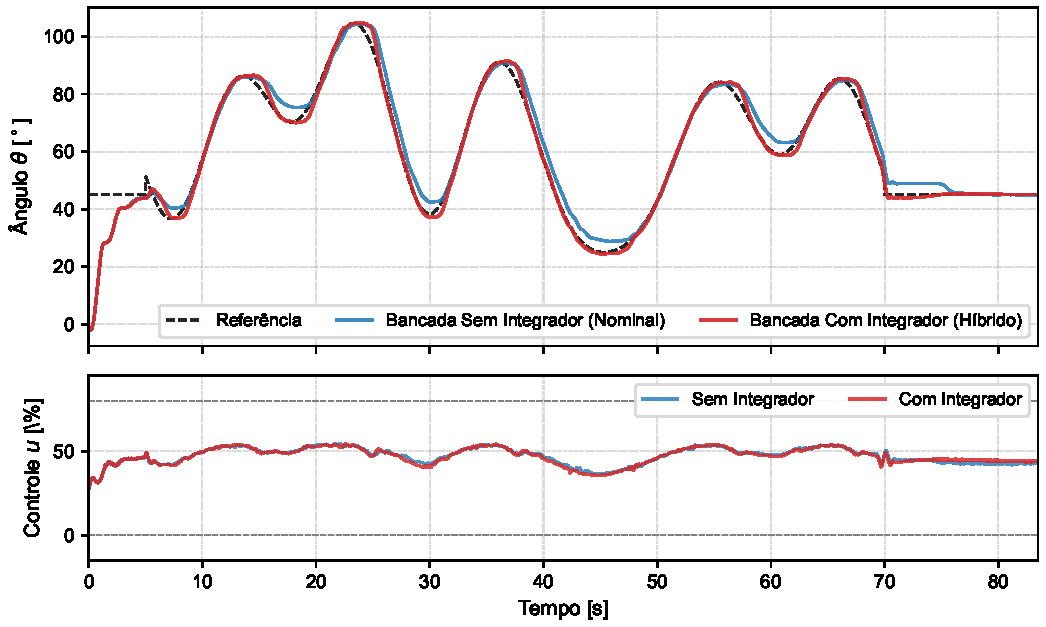
\includegraphics[width=8.4cm]{img/comparacao_hibrido_val3.pdf}
\caption{Physical bench response for Scenario 3 (Smooth Sine): mitigation of bearing stick-slip plateaus at velocity reversals by the Hybrid controller ($\mathrm{RMSE}$ reduced from $3.55^\circ$ to $1.75^\circ$).}
\label{fig:bench_hyb_val3}
\end{center}
\end{figure}

\subsection{Mirrored Comparison Against Classical PID Control}

To benchmark the embedded neural controller directly against the linear PID baseline on the physical bench, mirrored experiments were conducted using four demanding excitation trajectories at $\theta_0 = 45^\circ$ and $\theta_0 = 60^\circ$. Table~\ref{tb:pid_vs_ann} summarizes the tracking RMSE over both the full trial and the high-frequency steady-state window, while Fig.~\ref{fig:chirp45_pid_ann} depicts the time-domain response for the $\pm 35^\circ$ chirp trial.

\begin{table}[tb]
\begin{center}
\caption{Mirrored physical bench comparison (RMSE) between classical PID and Embedded Neural controller.}\label{tb:pid_vs_ann}
\resizebox{8.4cm}{!}{%
\begin{tabular}{llccc}
\toprule
\textbf{Excitation Profile} & \textbf{Window} & \textbf{PID ($^\circ$)} & \textbf{Neural ($^\circ$)} & \textbf{Improvement} \\
\midrule
Multisine $45^\circ$ ($0.50\,\mathrm{Hz}$) & Global ($0\text{--}80\,\mathrm{s}$) & $9.55$ & $\mathbf{2.16}$ & $-77.4\%$ \\
                                           & Steady ($20\text{--}60\,\mathrm{s}$)& $6.47$ & $\mathbf{1.99}$ & $-69.2\%$ \\
\midrule
Multisine $60^\circ$ ($0.50\,\mathrm{Hz}$) & Global ($0\text{--}80\,\mathrm{s}$) & $14.17$& $\mathbf{2.78}$ & $-80.4\%$ \\
                                           & Steady ($20\text{--}60\,\mathrm{s}$)& $12.55$& $\mathbf{2.51}$ & $-80.0\%$ \\
\midrule
Chirp $45^\circ$ ($\pm 35^\circ$)          & Global ($0\text{--}60\,\mathrm{s}$) & $15.81$& $\mathbf{2.94}$ & $-81.4\%$ \\
                                           & Steady ($10\text{--}60\,\mathrm{s}$)& $16.46$& $\mathbf{3.01}$ & $-81.7\%$ \\
\midrule
Chirp $60^\circ$ ($\pm 50^\circ$)          & Global ($0\text{--}60\,\mathrm{s}$) & $22.98$& $\mathbf{4.84}$ & $-78.9\%$ \\
                                           & Steady ($10\text{--}60\,\mathrm{s}$)& $26.02$& $\mathbf{4.82}$ & $-81.5\%$ \\
\bottomrule
\end{tabular}%
}
\end{center}
\end{table}

\begin{figure}[tb]
\begin{center}
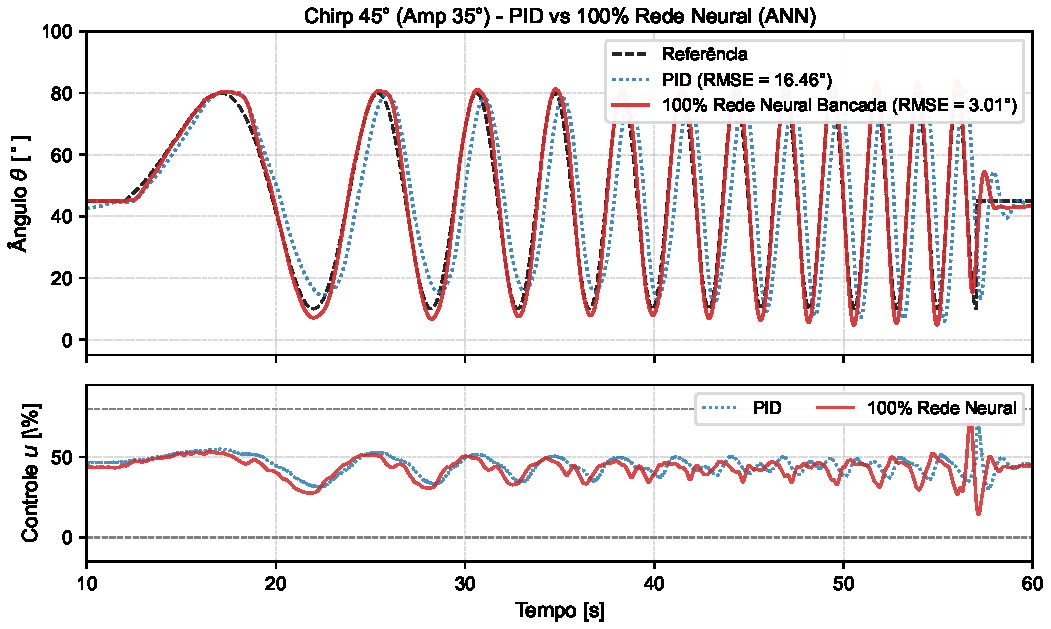
\includegraphics[width=8.4cm]{img/comparacao_rodada7_chirp45.pdf}
\caption{Mirrored bench tracking of a swept-sine chirp ($0.05\text{--}0.50\,\mathrm{Hz}$, $\pm 35^\circ$ around $45^\circ$): classical PID ($\mathrm{RMSE} = 16.46^\circ$) vs. Embedded Neural controller ($\mathrm{RMSE} = 3.01^\circ$).}
\label{fig:chirp45_pid_ann}
\end{center}
\end{figure}

As shown in Fig.~\ref{fig:chirp45_pid_ann} and Table~\ref{tb:pid_vs_ann}, the purely reactive PID controller suffers from severe phase lag ($>60^\circ\text{--}90^\circ$) as frequency approaches $0.50\,\mathrm{Hz}$, as well as static gain mismatch during wide angular excursions ($10^\circ$ to $110^\circ$ in the $60^\circ$ chirp, where PID RMSE reaches $26.02^\circ$). Conversely, by exploiting the $100$-step future reference preview and nonlinear NARX dynamics encoded during training, the neural controller decelerates the thruster ahead of trajectory peaks, maintaining strict phase synchronization and reducing tracking RMSE by $69.2\%$ to $81.7\%$.

\subsection{Embedded TinyML Optimization and Compression Analysis}

Deploying deep policies on low-cost microcontrollers requires balancing execution latency against Flash memory footprint. Using the hardware Data Watchpoint and Trace (DWT) cycle counter on the STM32F446RE ($180\,\mathrm{MHz}$ Cortex-M4F) over $8,365$ control cycles, we evaluated two deployment toolchains: (i)~native C matrix-vector routines compiled with ARM GCC under flags \texttt{-O0}, \texttt{-O1}, \texttt{-Os}, and \texttt{-O3}; and (ii)~the ST X-CUBE-AI code generator \citep{stmu2526,david2021} utilizing CMSIS-NN SIMD instructions, tested in both uncompressed \texttt{float32} and 4-bit non-linear LUT quantization (\emph{High Compression}).

\begin{table}[tb]
\begin{center}
\caption{Computational latency ($t_{\mathrm{ann}}$) and memory footprint on STM32F446RE ($180\,\mathrm{MHz}$, $T_s = 10\,\mathrm{ms}$).}\label{tb:tinyml_bench}
\resizebox{8.4cm}{!}{%
\begin{tabular}{lccccc}
\toprule
\textbf{Configuration} & \textbf{$t_{\mathrm{ann}}$ (ms)} & \textbf{CPU (\%)} & \textbf{Speedup} & \textbf{Weights Flash} & \textbf{Total Flash} \\
\midrule
Native C (\texttt{-O0})     & $10.07^*$ & $100.7\%^*$ & $1.00\times$ & $130.50\,\mathrm{KiB}$ & $183.05\,\mathrm{KB}$ \\
Native C (\texttt{-O1})     & $2.46$    & $24.6\%$    & $4.09\times$ & $130.50\,\mathrm{KiB}$ & $173.70\,\mathrm{KB}$ \\
Native C (\texttt{-Os})     & $2.08$    & $20.8\%$    & $4.84\times$ & $130.50\,\mathrm{KiB}$ & $174.14\,\mathrm{KB}$ \\
Native C (\texttt{-O3})     & $1.98$    & $19.8\%$    & $5.09\times$ & $130.50\,\mathrm{KiB}$ & $175.63\,\mathrm{KB}$ \\
\midrule
X-CUBE-AI (\texttt{float32})& $\mathbf{1.69}$ & $\mathbf{16.9\%}$ & $\mathbf{5.96\times}$ & $130.50\,\mathrm{KiB}$ & $182.25\,\mathrm{KB}$ \\
X-CUBE-AI (High Comp.)      & $\mathbf{1.82}$ & $\mathbf{18.2\%}$ & $\mathbf{5.53\times}$ & $\mathbf{17.75\,\mathrm{KiB}}$ & $\mathbf{69.51\,\mathrm{KB}}$ \\
\bottomrule
\multicolumn{6}{l}{\footnotesize $^*$Exceeds $T_s = 10\,\mathrm{ms}$ deadline, causing 1,878 cumulative sample overruns.}
\end{tabular}%
}
\end{center}
\end{table}

\begin{figure}[tb]
\begin{center}
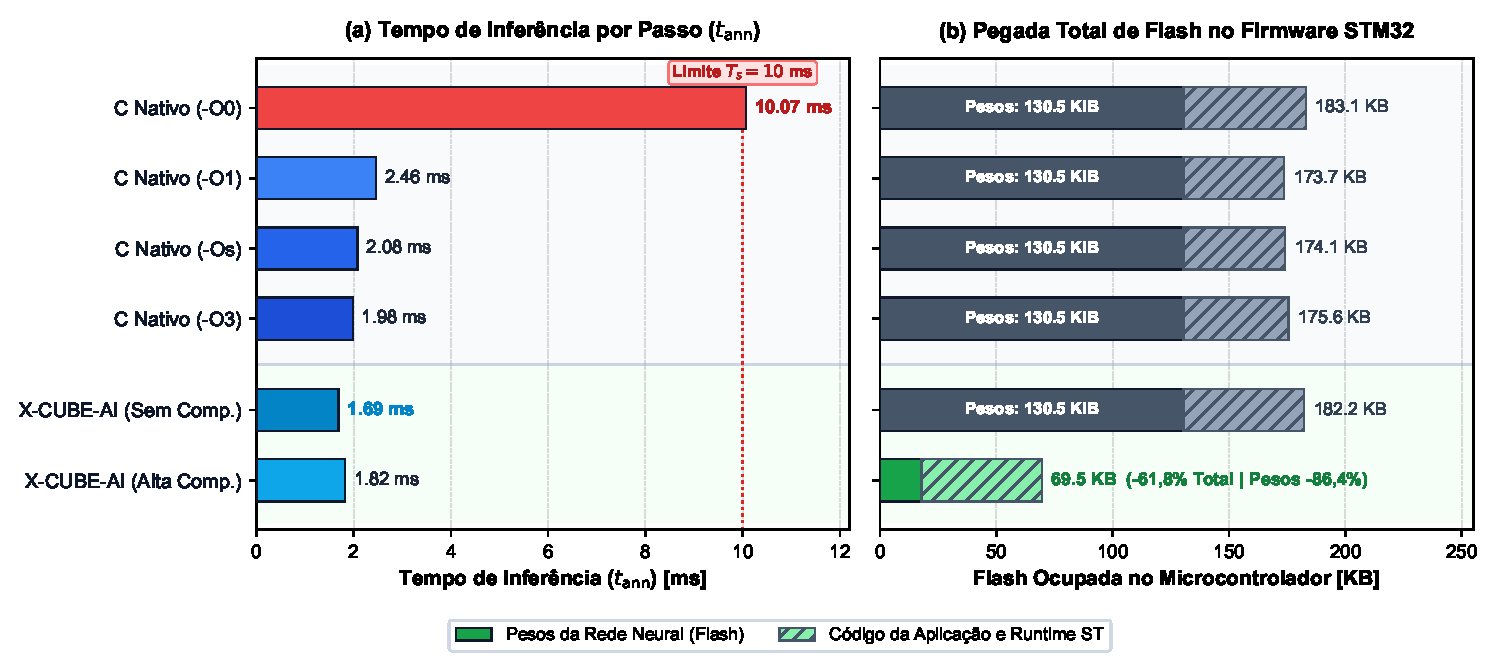
\includegraphics[width=8.4cm]{img/benchmark_inferencia_flash.pdf}
\caption{Comparison of per-step inference time ($t_{\mathrm{ann}}$) and Flash memory footprint across GCC optimization levels and ST X-CUBE-AI.}
\label{fig:tinyml_flash}
\end{center}
\end{figure}

The results in Table~\ref{tb:tinyml_bench} and Fig.~\ref{fig:tinyml_flash} highlight three key engineering findings:
\begin{enumerate}
    \item \textbf{Compiler Flags and Hard Real-Time Determinism:} Unoptimized compilation (\texttt{-O0}) requires $10.07\,\mathrm{ms}$, violating the $10\,\mathrm{ms}$ sampling deadline ($100.7\%$ CPU load). Enabling \texttt{-Os} or \texttt{-O3} reduces latency to $2.08\,\mathrm{ms}$ and $1.98\,\mathrm{ms}$ ($\sim 20\%$ CPU load) with sub-microsecond jitter ($< 1\,\mu\mathrm{s}$) due to the branch-free feedforward structure of the MLP.
    \item \textbf{SIMD Acceleration via X-CUBE-AI:} Uncompressed X-CUBE-AI achieves the fastest execution at $1.69\,\mathrm{ms}$ ($16.9\%$ CPU occupancy, $14.6\%$ faster than GCC \texttt{-O3}) by exploiting Cortex-M4 multiply-accumulate (MAC) pipeline scheduling, requiring only $2.78\,\mathrm{KiB}$ of RAM.
    \item \textbf{High Compression with Negligible Closed-Loop Impact:} Applying non-linear weight quantization shrinks weight storage by $\mathbf{86.4\%}$ ($130.50\,\mathrm{KiB} \to 17.75\,\mathrm{KiB}$) and total firmware size by $61.8\%$ ($182.25\,\mathrm{KB} \to 69.51\,\mathrm{KB}$), while adding only $0.13\,\mathrm{ms}$ of runtime LUT decoding overhead ($t_{\mathrm{ann}} = 1.82\,\mathrm{ms}$, still $8.1\%$ faster than native C \texttt{-O3}). Closed-loop SIL tests on Scenario~1 confirmed that the compressed model preserves stability and transient fidelity, shifting active-window RMSE by only $+0.38^\circ$ ($1.53^\circ \to 1.91^\circ$) and global RMSE by $+0.11^\circ$ ($4.88^\circ \to 5.00^\circ$), making the neural NMPC deployable even on ultra-low-cost microcontrollers with $64\,\mathrm{KB}$ of Flash.
\end{enumerate}

%===============================================================================
\section{Conclusion}
\label{sec:conclusion}

This paper presented the design, TinyML deployment, and experimental validation of an embedded neural predictive controller for a 1-DOF quarter-drone aeropendulum operating at $100\,\mathrm{Hz}$. By identifying a compact 10-term polynomial NARX model via FROLS and distilling a long-horizon CasADi/IPOPT NMPC policy ($N = 150$) with future reference preview into a $130 \to 128 \to 128 \to 1$ ReLU MLP, the computational bottleneck of online NLP optimization ($90\text{--}458\,\mathrm{ms}$) was reduced to a deterministic $1.69\text{--}2.08\,\mathrm{ms}$ feedforward execution on an STM32F446RE microcontroller.

Furthermore, coupling the neural policy with a bounded parallel residual integrator ($\pm 10\%$ authority) effectively bridged the Sim-to-Real gap on the physical bench, attenuating steady-state offset by $96.2\%$ to $98.8\%$ and mitigating bearing stick-slip friction to reduce sinusoidal tracking RMSE by $50.8\%$. Mirrored experimental trials against a classical PID controller demonstrated $69.2\%$ to $81.7\%$ reductions in tracking RMSE across aggressive multisine and chirp trajectories. Finally, X-CUBE-AI weight quantization compressed parameter Flash usage by $86.4\%$ ($17.75\,\mathrm{KiB}$) at $1.82\,\mathrm{ms}$ latency with negligible closed-loop degradation.

Future work will investigate iterative dataset aggregation (DAgger) \citep{ross2011reduction} to mitigate distribution shift at extreme angles, full 8-bit integer quantization (INT8) \citep{jacob2018quantization} for FPU-less Cortex-M0+ processors, and extension to multi-DOF VTOL attitude control.

\bibliography{ifacconf}

\end{document}
